\section{Sharing Data Between Clusters with \textsc{Charon}}

An innovative aspect of the BiobankCloud PaaS is the capability of interconnect several PaaS deployments in a cloud federation~\cite{ebb13}. This enables data sharing and allows the use of public clouds (e.g., Amazon S3, Google Storage) for storing data. This interconnection is implemented through a novel storage system called \textsc{Charon}.

\textsc{Charon} is a cloud-backed file system capable of storing and sharing big data in a secure and reliable way using multiple cloud providers and storage repositories. It is secure and reliable because it does not require trust on any single provider, and it supports the storage of different data sets in distinct locations to comply with required privacy premises. Two distinguishing features of \textsc{Charon} are its \emph{serverless design} (no client-managed server is required in the cloud) and its \emph{efficient management of large files} (by employing prefetching, cache, compression and background writes).
Figure~\ref{fig:charon} illustrates a deployment scenario where two biobanks store their data in local repositories (e.g., HopsFS), in single public cloud providers, and in a resilient cloud-of-clouds~\cite{depsky13}. In this scenario, the namespace tree has six nodes: directories \texttt{d1} and \texttt{d2}, and files \texttt{A}, \texttt{B}, \texttt{C}, and \texttt{D}. 
The namespace is maintained in the cloud-of-clouds, together with file \texttt{B}.
File \texttt{D}, less critical, is kept in a single cloud.
File \texttt{A} is stored locally because it cannot leave Biobank 2.
File \texttt{C} is shared between the two sites (e.g., in the same country), thus being stored in both of them.

\begin{figure}[ht]
 \centering
 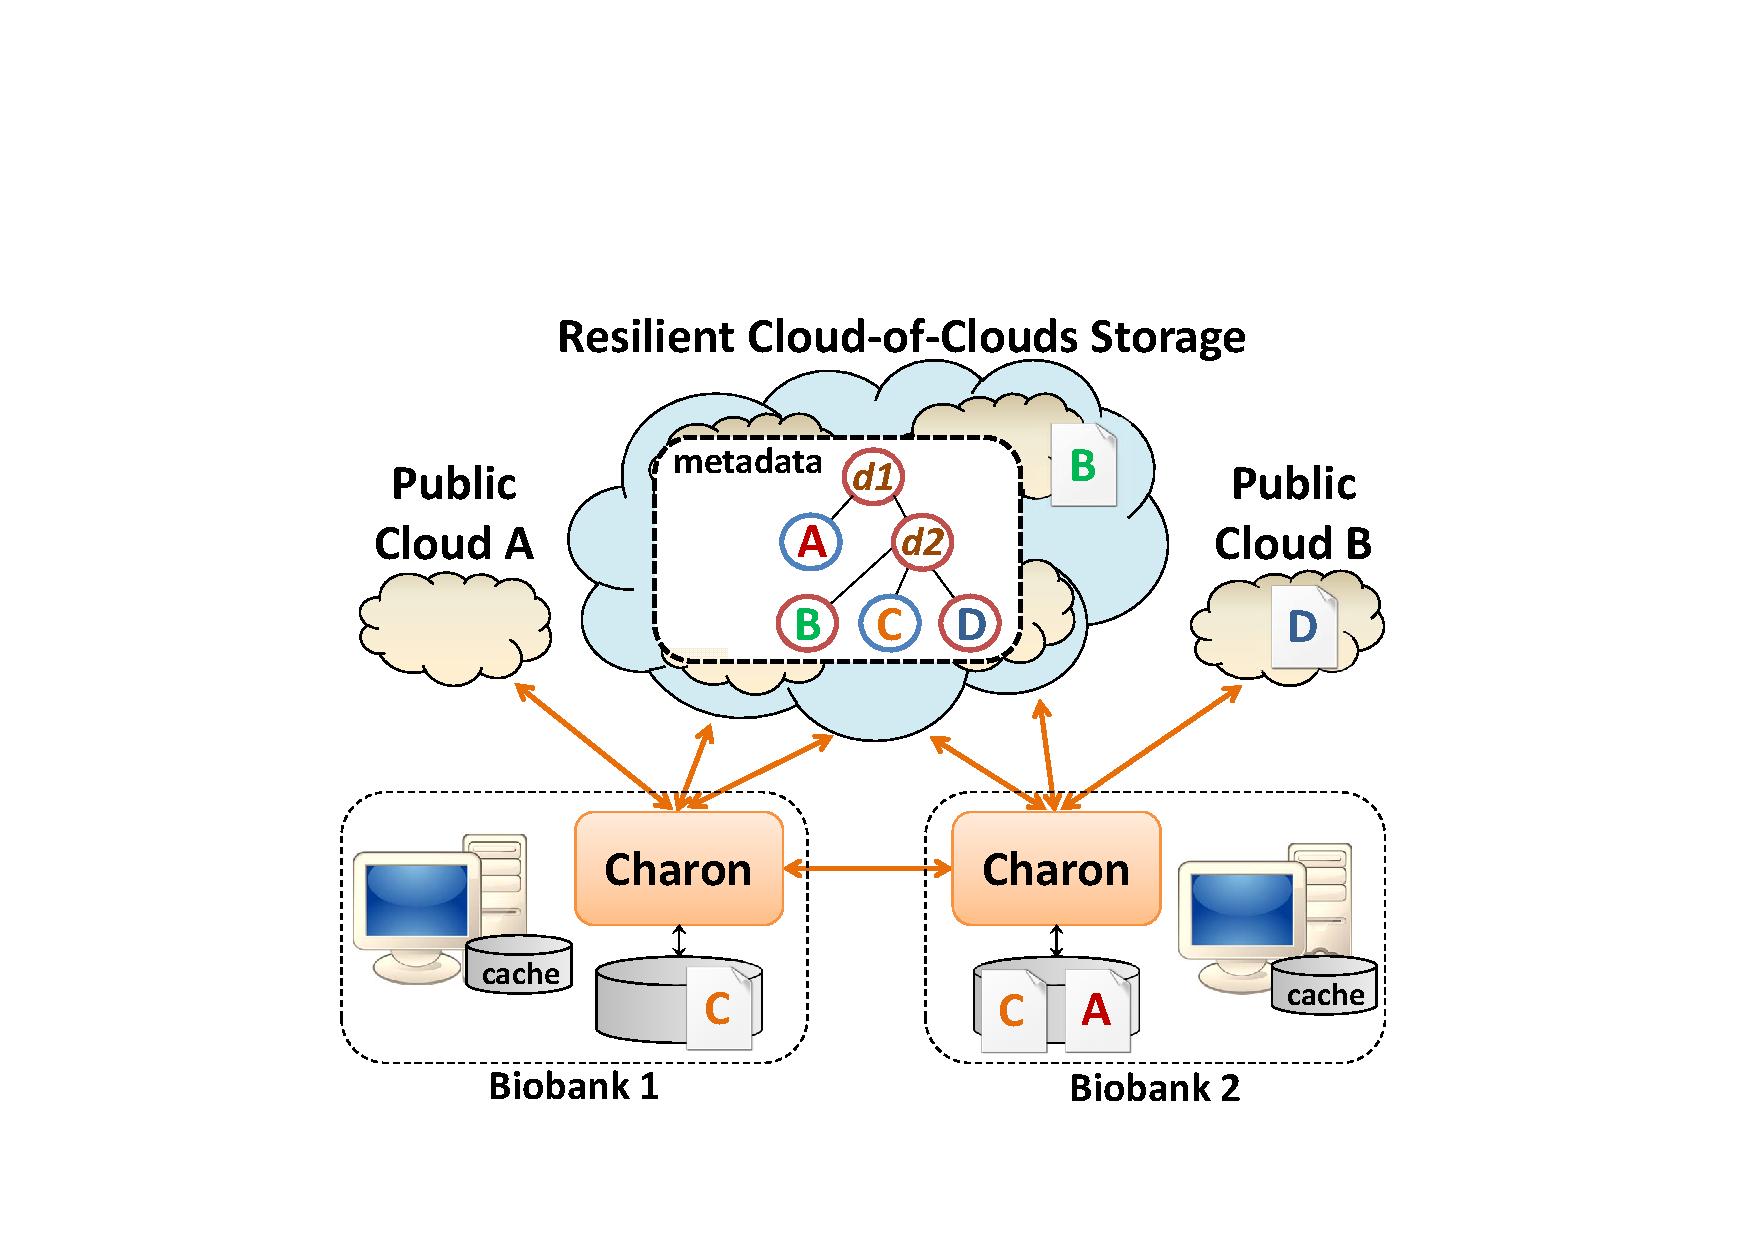
\includegraphics[width=0.5\columnwidth]{./imgs/charon_arch.pdf}
 % charon_arch.pdf: 0x0 pixel, 300dpi, 0.00x0.00 cm, bb=
\caption{\small \textsc{Charon} overview.}
\label{fig:charon}
\end{figure}
